\documentclass{article}
\title{The thick data}
\usepackage{graphicx}
\usepackage{Statweave}
\begin{document}
\maketitle
The data:
\begin{verbatim}
\end{verbatim}
The SAS code and output:
\begin{Winput}
options linesize=70;

data thick; 
  input east north thick @@;
  datalines; 
   0.7  59.6  34.1   2.1  82.7  42.2   4.7  75.1  39.5  
   4.8  52.8  34.3   5.9  67.1  37.0   6.0  35.7  35.9 
   6.4  33.7  36.4   7.0  46.7  34.6   8.2  40.1  35.4    
  13.3   0.6  44.7  13.3  68.2  37.8  13.4  31.3  37.8 
  17.8   6.9  43.9  20.1  66.3  37.7  22.7  87.6  42.8  
  23.0  93.9  43.6  24.3  73.0  39.3  24.8  15.1  42.3 
  24.8  26.3  39.7  26.4  58.0  36.9  26.9  65.0  37.8  
  27.7  83.3  41.8  27.9  90.8  43.3  29.1  47.9  36.7 
  29.5  89.4  43.0  30.1   6.1  43.6  30.8  12.1  42.8 
  32.7  40.2  37.5  34.8   8.1  43.3  35.3  32.0  38.8 
  37.0  70.3  39.2  38.2  77.9  40.7  38.9  23.3  40.5 
  39.4  82.5  41.4  43.0   4.7  43.3  43.7   7.6  43.1 
  46.4  84.1  41.5  46.7  10.6  42.6  49.9  22.1  40.7 
  51.0  88.8  42.0  52.8  68.9  39.3  52.9  32.7  39.2 
  55.5  92.9  42.2  56.0   1.6  42.7  60.6  75.2  40.1 
  62.1  26.6  40.1  63.0  12.7  41.8  69.0  75.6  40.1 
  70.5  83.7  40.9  70.9  11.0  41.7  71.5  29.5  39.8 
  78.1  45.5  38.7  78.2   9.1  41.7  78.4  20.0  40.8 
  80.5  55.9  38.7  81.1  51.0  38.6  83.8   7.9  41.6 
  84.5  11.0  41.5  85.2  67.3  39.4  85.5  73.0  39.8  
  86.7  70.4  39.6  87.2  55.7  38.8  88.1   0.0  41.6 
  88.4  12.1  41.3  88.4  99.6  41.2  88.8  82.9  40.5  
  88.9   6.2  41.5  90.6   7.0  41.5  90.7  49.6  38.9  
  91.5  55.4  39.0  92.9  46.8  39.1  93.4  70.9  39.7  
  94.8  71.5  39.7  96.2  84.3  40.3  98.2  58.2  39.5 
;

proc g3d;
    scatter north*east=thick;

proc plot vpercent=50;
    plot north*east=thick / contour=5;
\end{Winput}
\begin{Woutput}
                     Contour plot of north*east.
north |
  100 +                                                      W
      |               #  ##              W
      |  W            #  W      W   W  W          W          W    W
      |    X                   W            W    W
      |         X      X      X         X                  XX   XX
      |     +       X   X                                  X
      | .               +                               X   X  X   X
   50 +    ..            +                               X    X X
      |      +              X                          X
      |     +                           X
      |         X      X     X               W     X
      |                        W      W                W
      |                W  #                   W    W       W W
      |            #      #  #    # #                  W  W  WW
    0 +         #                         #                  W
      --+-----------+-----------+-----------+-----------+-----------+-
        0          20          40          60          80          100
                                    east
 Symbol        thick     Symbol        thick     Symbol        thick
 .....   32.5 - 35.0     XXXXX   37.5 - 40.0     #####   42.5 - 45.0
 +++++   35.0 - 37.5     WWWWW   40.0 - 42.5
NOTE: 2 obs hidden.
\end{Woutput}
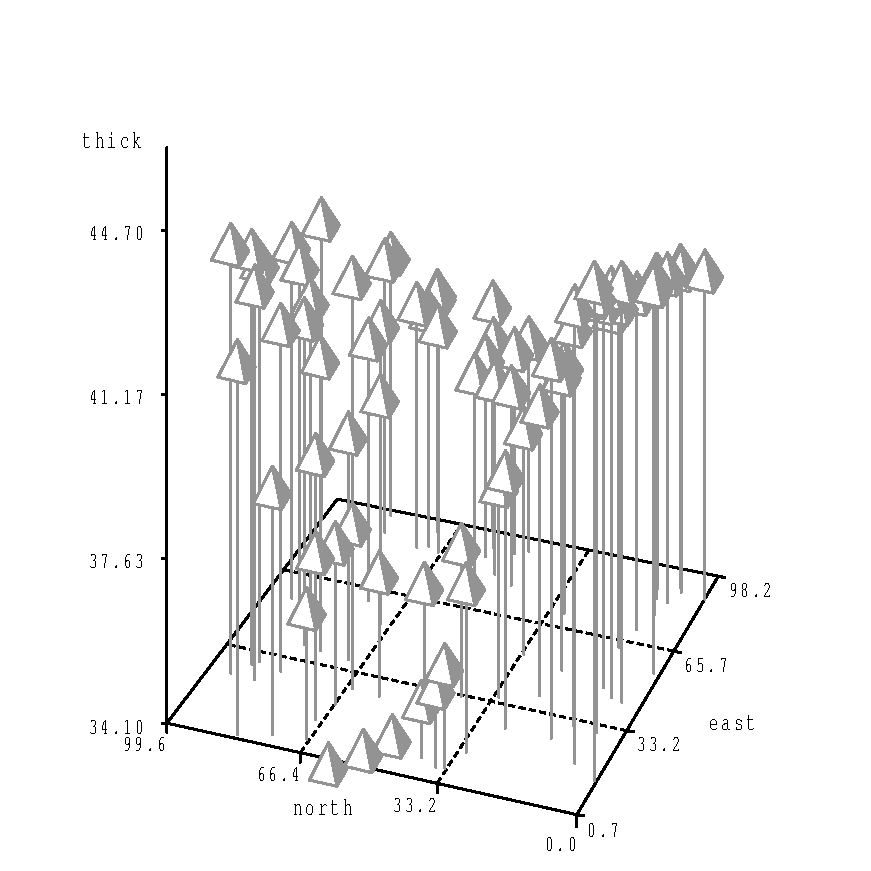
\includegraphics[]{thick-1-SAS-fig.pdf}

\begin{Winput}
proc variogram;
    compute novariogram;
    coordinates xc=east yc=north;
    var thick;

proc variogram;
    compute nhclasses=30 novariogram;
    coordinates xc=east yc=north;
    var thick;

proc variogram data=thick outv = outv; 
  compute lagd = 5 maxlag = 20; 
  coordinates xc=east yc=north; 
  var thick;

proc print;

proc gplot;
    plot variog*distance;
\end{Winput}
\begin{Woutput}
The VARIOGRAM Procedure
Dependent Variable: thick
Number of Observations Read          75
Number of Observations Used          75

              Pairs Information
Number of Lags                              11
Lag Distance                             13.94
Maximum Data Distance in east            97.50
Maximum Data Distance in north           99.60
Maximum Data Distance                   139.38

               Pairwise Distance Intervals
                                     Number
  Lag                                    of    Percentage
Class    ---------Bounds---------     Pairs      of Pairs
    0          0.00          6.97        45        1.62%
    1          6.97         20.91       263        9.48%
    2         20.91         34.84       383       13.80%
    3         34.84         48.78       436       15.71%
    4         48.78         62.72       495       17.84%
    5         62.72         76.66       525       18.92%
    6         76.66         90.60       412       14.85%
    7         90.60        104.53       179        6.45%
    8        104.53        118.47        35        1.26%
    9        118.47        132.41         2        0.07%
   10        132.41        146.35         0        0.00%

The VARIOGRAM Procedure
Dependent Variable: thick
Number of Observations Read          75
Number of Observations Used          75

              Pairs Information
Number of Lags                              31
Lag Distance                              4.65
Maximum Data Distance in east            97.50
Maximum Data Distance in north           99.60
Maximum Data Distance                   139.38

               Pairwise Distance Intervals
                                     Number
  Lag                                    of    Percentage
Class    ---------Bounds---------     Pairs      of Pairs
    0          0.00          2.32         4        0.14%
    1          2.32          6.97        41        1.48%
    2          6.97         11.61        69        2.49%
    3         11.61         16.26        86        3.10%
    4         16.26         20.91       108        3.89%
    5         20.91         25.55       120        4.32%
    6         25.55         30.20       139        5.01%
    7         30.20         34.84       124        4.47%
    8         34.84         39.49       128        4.61%
    9         39.49         44.14       143        5.15%
   10         44.14         48.78       165        5.95%
   11         48.78         53.43       146        5.26%
   12         53.43         58.07       140        5.05%
   13         58.07         62.72       209        7.53%
   14         62.72         67.37       184        6.63%
   15         67.37         72.01       170        6.13%
   16         72.01         76.66       171        6.16%
   17         76.66         81.30       149        5.37%
   18         81.30         85.95       150        5.41%
   19         85.95         90.60       113        4.07%
   20         90.60         95.24        89        3.21%
   21         95.24         99.89        60        2.16%
   22         99.89        104.53        30        1.08%
   23        104.53        109.18        19        0.68%
   24        109.18        113.83        11        0.40%
   25        113.83        118.47         5        0.18%
   26        118.47        123.12         1        0.04%
   27        123.12        127.76         1        0.04%
   28        127.76        132.41         0        0.00%
   29        132.41        137.06         0        0.00%
   30        137.06        141.70         0        0.00%

The VARIOGRAM Procedure
Dependent Variable: thick
Number of Observations Read          75
Number of Observations Used          75

The VARIOGRAM Procedure
Dependent Variable: thick
        Empirical Semivariogram
  Lag      Pair     Average
Class     Count    Distance     Semivariance
    0         4        1.89     0.0425
    1        51        5.94     0.1236
    2        76       10.17     0.7024
    3       104       15.12     1.3100
    4       123       20.15     2.7324
    5       136       25.31     4.0214
    6       130       29.87     5.1648
    7       150       35.06     5.8808
    8       137       40.18     7.6515
    9       163       45.03     6.9541
   10       165       49.70     7.4056
   11       159       54.88     7.3282
   12       219       60.10     7.1324
   13       194       65.10     6.3167
   14       180       69.93     5.8192
   15       190       74.93     5.4322
   16       155       80.11     5.3506
   17       151       85.03     5.1577
   18       117       89.90     6.0803
   19        73       94.66     7.6629
   20        47       99.54     6.6128

Obs VARNAME LAG COUNT DISTANCE AVERAGE  VARIOG  STDERR   COVAR
  1  thick   -1   75     .     40.1387  .       .       5.59592
  2  thick    0    4    1.8919 40.1250 0.04250 0.03005  6.73456
  3  thick    1   51    5.9367 40.4382 0.12363 0.02448  5.54671
  4  thick    2   76   10.1651 40.0428 0.70243 0.11395  3.72434
  5  thick    3  104   15.1243 40.1115 1.31000 0.18166  3.29897
  6  thick    4  123   20.1472 40.0516 2.73240 0.34842  2.68629
  7  thick    5  136   25.3109 39.8081 4.02140 0.48767  1.88510
  8  thick    6  130   29.8661 39.8746 5.16485 0.64062  0.64092
  9  thick    7  150   35.0573 39.8130 5.88077 0.67905 -0.51211
 10  thick    8  137   40.1762 39.9540 7.65146 0.92448 -1.93853
 11  thick    9  163   45.0273 39.8837 6.95408 0.77030 -1.85804
 12  thick   10  165   49.6994 39.8558 7.40564 0.81533 -2.31356
 13  thick   11  159   54.8782 39.8881 7.32824 0.82189 -2.23589
 14  thick   12  219   60.0973 40.0637 7.13244 0.68160 -2.08081
 15  thick   13  194   65.1025 40.2987 6.31673 0.64137 -1.71279
 16  thick   14  180   69.9306 40.2514 5.81919 0.61340 -0.91277
 17  thick   15  190   74.9328 40.3763 5.43221 0.55733  0.05297
 18  thick   16  155   80.1055 40.4206 5.35065 0.60779  0.36238
 19  thick   17  151   85.0293 40.4940 5.15768 0.59358  1.69427
 20  thick   18  117   89.9044 40.2175 6.08030 0.79496  0.98993
 21  thick   19   73   94.6578 40.1733 7.66295 1.26838  0.18459
 22  thick   20   47   99.5352 40.8447 6.61277 1.36411  0.30689
\end{Woutput}
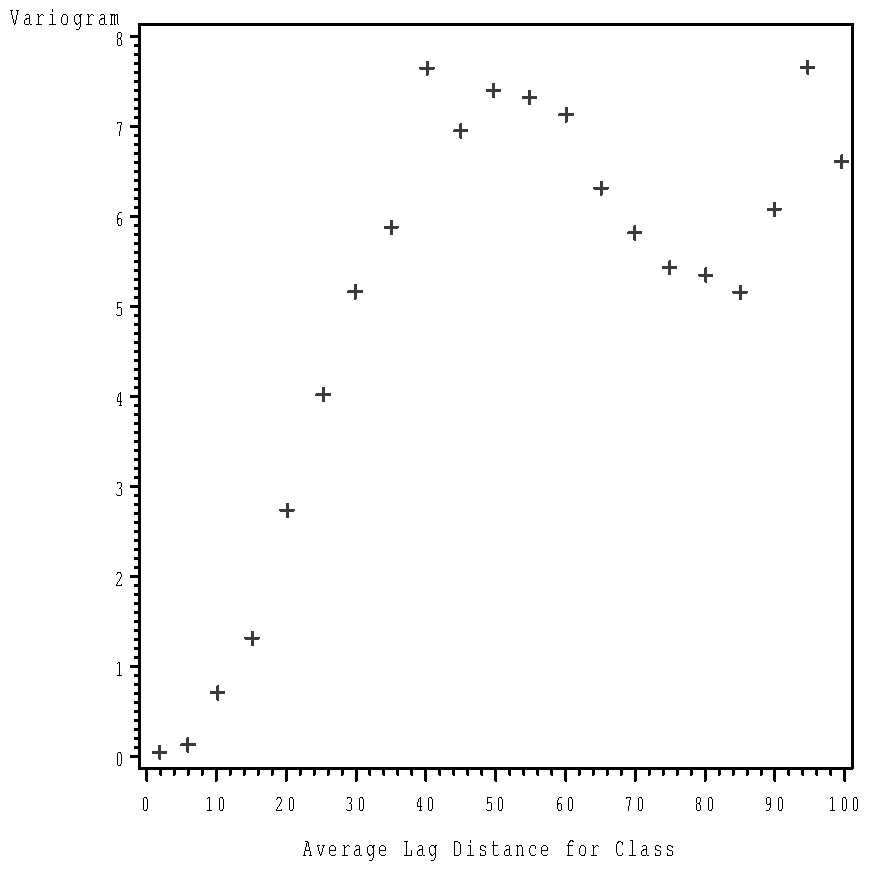
\includegraphics[]{thick-2-SAS-fig.pdf}

\begin{Winput}
proc krige2d data=thick outest=est; 
  coord xc=east yc=north; 
  grid x=0 to 100 by 5 y=0 to 100 by 5; 
  pred var=thick r=10; 
  model scale=7 range=30 form=gauss; 

proc print data = est (obs = 10); 

proc g3d data=est;
  plot gyc*gxc=estimate;
  label gyc      = 'North' 
        gxc      = 'East' 
        estimate = 'Estimated Thickness'; 
\end{Winput}
\begin{Woutput}
The KRIGE2D Procedure
Dependent Variable: thick
Number of Observations Read          75
Number of Observations Used          75

                  Kriging Information
Prediction Grid Points                               441
Type of Analysis                                   Local
Neighborhood Search Radius                            10
Grid Points with Radius Incremented                  441
Maximum Radius                                 56.048283
Minimum Neighbors                                     20
Maximum Neighbors                      All Within Radius

The KRIGE2D Procedure
Dependent Variable: thick
Prediction: Pred1, Model: Model1
Covariance Model Information
Type                Gaussian
Sill                       7
Range                     30
Effective Range    51.961524
Nugget Effect              0

Obs     LABEL      VARNAME  GXC  GYC  NPOINTS  ESTIMATE   STDERR
  1  Pred1.Model1   thick    0     0     20     44.0107  0.66714
  2  Pred1.Model1   thick    0     5     20     43.3504  0.65143
  3  Pred1.Model1   thick    0    10     20     42.3169  0.59026
  4  Pred1.Model1   thick    0    15     20     40.9308  0.52172
  5  Pred1.Model1   thick    0    20     20     39.4097  0.36240
  6  Pred1.Model1   thick    0    25     20     37.8804  0.22627
  7  Pred1.Model1   thick    0    30     20     36.3949  0.15932
  8  Pred1.Model1   thick    0    35     20     35.2236  0.10873
  9  Pred1.Model1   thick    0    40     20     33.9929  0.06815
 10  Pred1.Model1   thick    0    45     20     33.2266  0.05748
\end{Woutput}
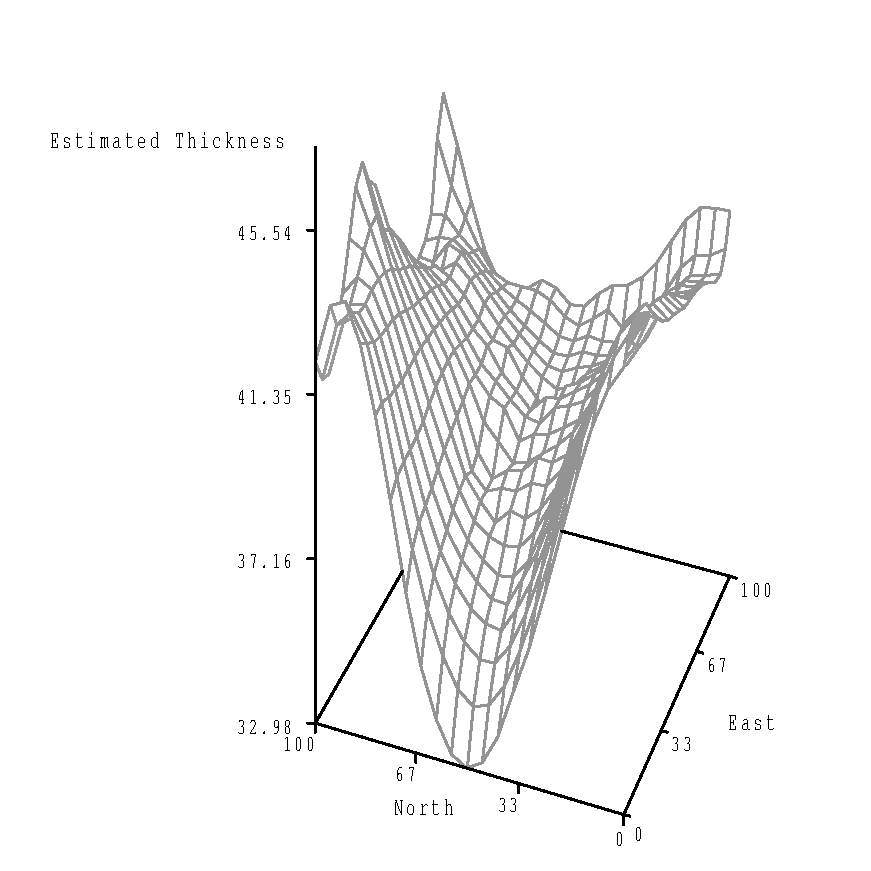
\includegraphics[]{thick-3-SAS-fig.pdf}

\begin{Winput}
proc gcontour data=est;
    plot gyc*gxc=estimate / nlevels=10 autolabel;
  label gyc      = 'North' 
        gxc      = 'East' 
        estimate = 'Estimated Thickness'; 
\end{Winput}
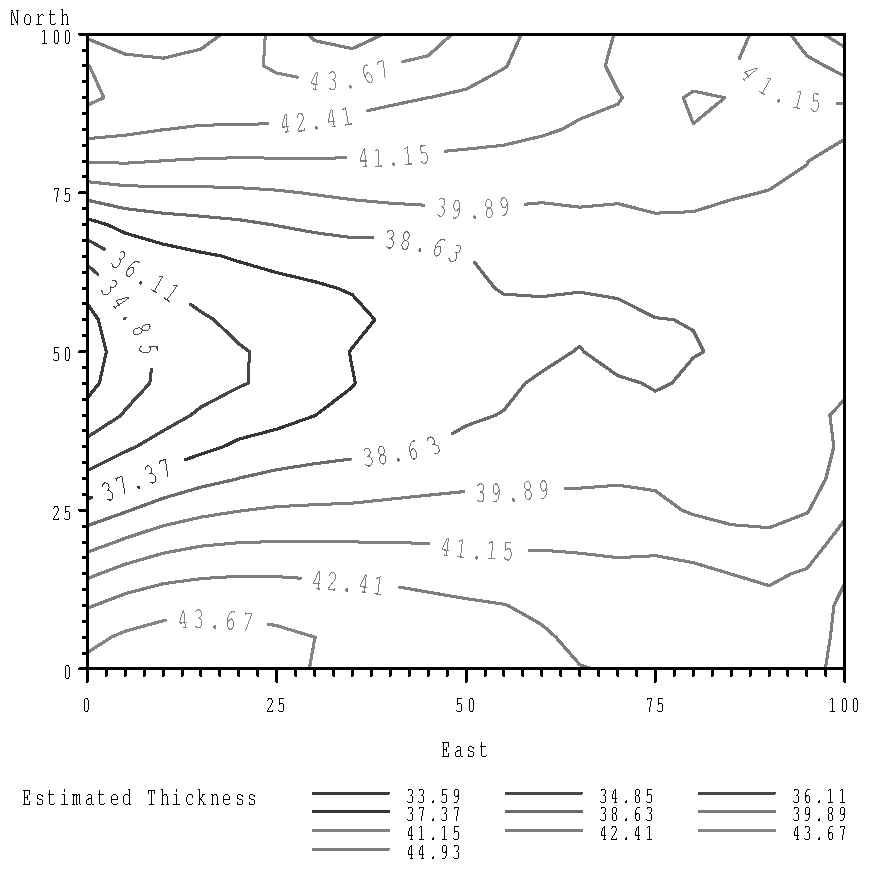
\includegraphics[]{thick-4-SAS-fig.pdf}

\begin{Winput}
proc gcontour data=est;
    plot gyc*gxc=stderr / nlevels=5 autolabel;
  label gyc      = 'North' 
        gxc      = 'East' 
        estimate = 'SE of Est Thickness'; 


    
run;
\end{Winput}
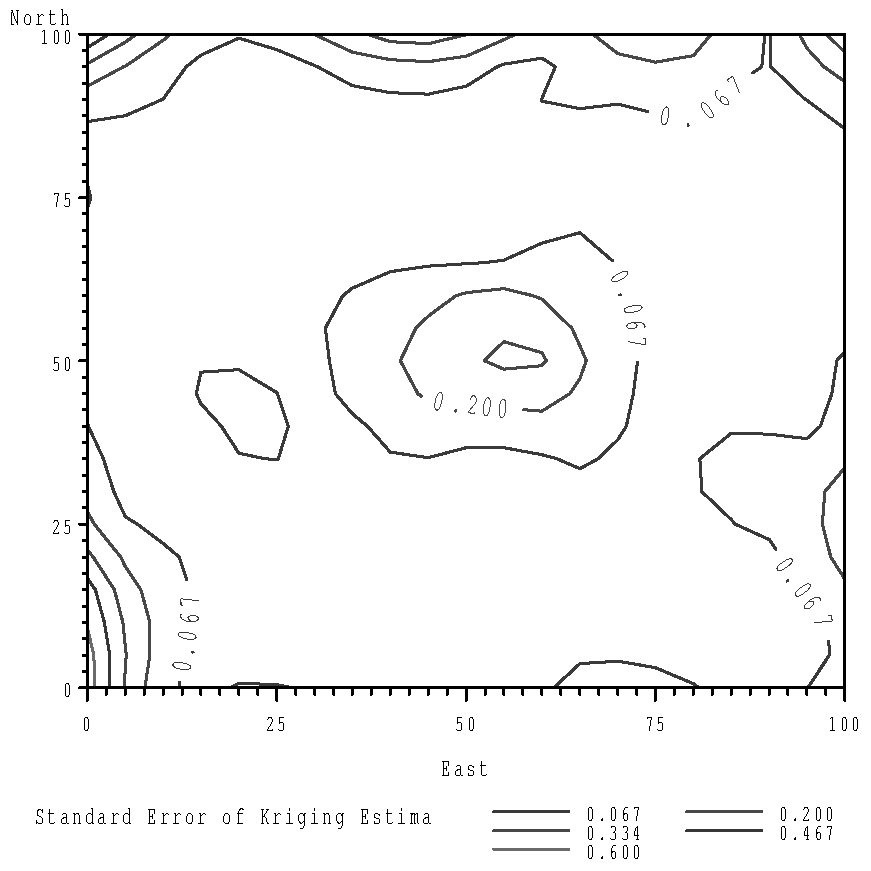
\includegraphics[]{thick-5-SAS-fig.pdf}
\end{document}
